The hybrid system outlined in Chapter~\ref{chap:Hybrid_Cache} introduces the
concept of data eviction. While in previous implementations the cache grows
incrementally without eviction, here we explore the potential of a cache that
removes data as it approaches its maximum capacity. This implementation can be
used individually or as part of a cooperative cache and provides a tuning
parameter that can be used to improve the cost efficiency of applications.

\section{First-In First-Out} % (fold)
\label{sec:fifo}
One of the most simple eviction systems we explore is that of a First-In
First-Out (FIFO) queue. This ubiquitous queue processing technique operates
just as the name suggest: those elements added into the queue first are also
the first to be removed. As detailed in Section~\ref{sub:hybrid_insert}, in our
system, each key is additionally placed into a priority queue on insertion. Once
the system reaches overflow capacity, eviction begins by dequeuing items from
the priority queue. With a FIFO technique this creates a temporal relationship
between cache inserts and cache hits. We expect that this configuration will
work most advantageously with workloads that frequently request data after its
initial insertion. For example: we expect FIFO to work best in scientific
workflows where component subcomputations are to be reused in many further
computations that immediately follow.

% section fifo (end)

\section{Least Recently Used} % (fold)
\label{sec:lru}
In addition to FIFO, we implement a form of cache algorithm that falls into the
family known as Least Recently Used (LRU)\cite{lru}. As the name implies, this
algorithm discards elements that have not been referenced for the longest time.
This somewhat approximates an optimal eviction algorithm, in that the optimal
algorithm will discard those elements that \emph{will} be used the furthest in
the \emph{future}. Comparatively, LRU discards those elements that \emph{were}
used furthest in the \emph{past}. We use this structure due to its wide spread
popularity, near-optimal performance, and the ease of implementation.

Unfortunately, LRU comes with its own issues that often prevent it from being
used in production. Computationally, maintaining the structure becomes quite
complex at higher levels of
associativity\cite{zhang_cache_schemes,deville_replacement}. One of the ways
to implement LRU involves maintaining a counter for each data element.
Whenever an element is referenced, the current time is stored in the table
entry for that key. When it comes time to evict, the elements with the smallest
time values, or those furthest in the past, are removed first. This does
however mean performing a linear search over the table to find the oldest
entries for each eviction. This is a very expensive operation when eviction
occurs frequently. A similar implementation may use a heap-based priority
queue, however, in order to find and update the timestamp this takes $O(n)$
time (for search) in addition to possible rebalances of the heap as a whole.

One of the other means of implementation, and the one we use for our
experiments, involves using a simple FIFO queue. On each update or retrieval,
the key is first removed from the queue before being pushed onto the end. In
this way, the oldest data elements are the first to be shifted out. Although
this means a data element must be found and deleted before being reinserted
each and every update, there is no data storage overhead associated with the
collection and maintenance of timestamps. Since this system is a cache in which
memory is at a premium, we choose to implement this more computationally
expensive algorithm.

\begin{algorithm}[htp]
\small
\caption{\label{alg:lru_store}lru\_store($key$)}
\begin{algorithmic}[1]
\STATE $\triangleright$ Obtain the global eviction queue $lru$

\STATE $\triangleright$ Identify the index at which the key resides
\IF{$index\ \leftarrow lru$.index($key$)}
  \STATE $lru$.delete\_at($index$)
\ENDIF
\STATE $lru$.push($key$)
\end{algorithmic}
\end{algorithm}

\begin{algorithm}[htp]
\small
\caption{\label{alg:lru_update}lru\_update($key$)}
\begin{algorithmic}[1]
\STATE $\triangleright$ Obtain the global eviction queue $lru$

\STATE $\triangleright$ Identify the index at which the key resides
\IF{$index\ \leftarrow lru$.index($key$)}
  \STATE $lru$.delete\_at($index$)
  \STATE $lru$.push($key$)
\ENDIF
\end{algorithmic}
\end{algorithm}

Algorithms~\ref{alg:lru_store} and~\ref{alg:lru_update} both operate in a very
similar manner. In both cases, the key is first removed from the queue before
reinserting it onto the end. The difference between the two is the location of
the reinsert: \emph{lru\_store} always inserts the new data element while
\emph{lru\_update} only inserts the data element if it was there previously.
For our purposes, \emph{lru\_store} is called during cache insertion, when new
keys are potentially being added into the queue, while \emph{lru\_update} is
called during cache searches when new, previously nonexistent elements should
not be inserted into the queue.

% section lru (end)

\section{Persistence} % (fold)
\label{sec:persistence}
In addition to eviction mechanisms, here we explore the impact of the eviction
methods both with and without a persistent storage mechanism. As in the
previous chapter, we do of course expect the systems with S3 support to
outperform those without given the same experiment options. However, we also
wish to see how persistence affects the cache under differing query patterns
for different eviction types.

Recall from section~\ref{sub:hybrid_insert} that data is evicted from memory
into the persistent storage medium. Eviction is controlled by one of the two
previously mentioned algorithms.

% section persistence (end)

\section{Experiments} % (fold)
\label{sec:experiments_eviction}
For these experiments we deploy a configuration designed to test our cache
server implementation. To do so, we distinguish between the server node
(running the server application) and the experiment broker. The experiment
broker handles launching the server instance, establishes a connection, and
then proceeds to run a series of specified tests. Since the following tests are
crafted to assess the performance of individual nodes rather than the entire
system, the experiment broker does not handle more than one node and data is
never migrated between nodes. This layout can be seen in
Figure~\ref{fig:experiment_layout}.

For each query, the experiment broker starts initially by executing a search on
the key. If the server can retrieve that data, it indicates a successful search
and proceeds to send it to the experiment broker. This is considered a
successful hit. If the server is \emph{unable} to retrieve said data, it
indicates a cache miss and a penalty of 75 seconds is applied to the total
running time to simulate the amount of time it would take to compute such data
(recall from Figure~\ref{fig:architecture} that a cache miss results in service
execution). The experiment broker then proceeds to insert the data into the
cache, at which point the cache may decide to evict. In every eviction, the
cache evicts 10\% of the total number of keys it may contain (i.e. 200 keys are
evicted with a threshold size of 2000).

\begin{figure}[htp]
\begin{center}
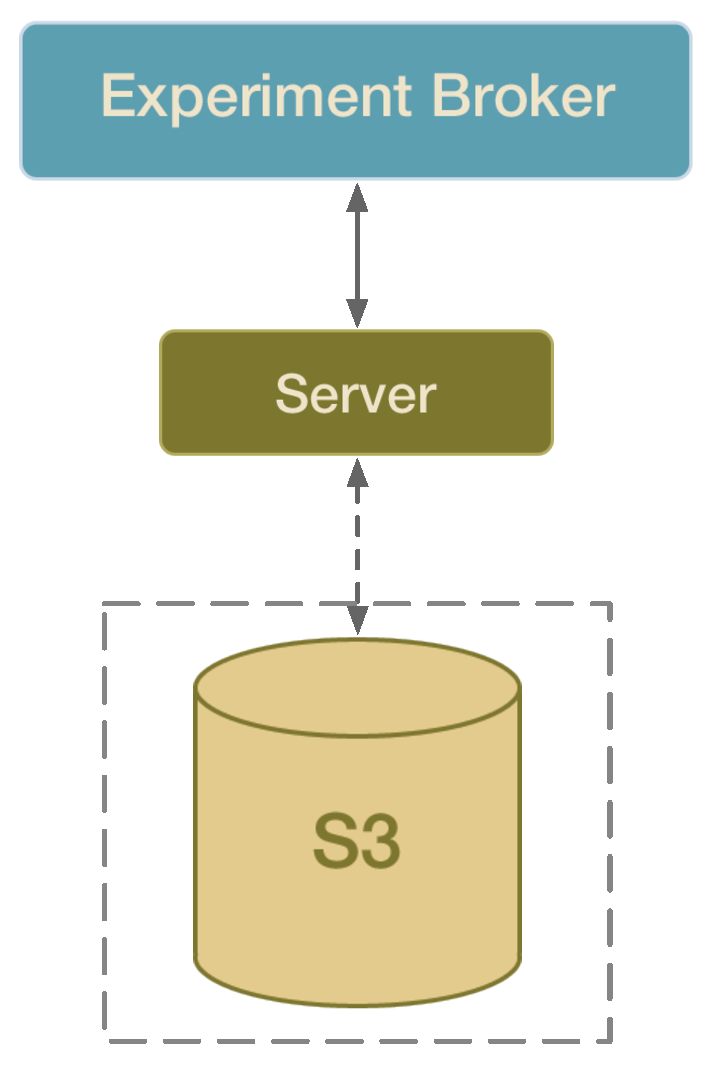
\includegraphics[scale=0.4]{figures/experiment_setup.pdf}
\end{center}
\caption{Experiment Layout}
\label{fig:experiment_layout}
\end{figure}

Each server node is running on a 64-bit Ubuntu 10.10 image using Ruby 1.9.2p180
(MRI). Each image is launched on an \emph{Extra Large instance} ({\tt
m1.xlarge}), which, by Amazon's specifications contains 15GB of memory, 8 EC2
compute units (each compute unit is equivalent to a 1.0-1.2GHz 2007 Xeon or
2007 Opteron processor) and has ``high'' I/O performance. For all experiments
the cache starts cold and both the indices and data are stored in memory.

For our experiments we simulate two different data sets and eight different
experimental configurations, for a total of 16 experiments. Our data sets vary
in a few regards: size, the number of key-value pairs to be stored in the cache
(\emph{threshold}), the total number of keys used across the queries, and the
number of queries.

One data set (the first row of Table~\ref{tab:data_types}) is designed such
that there are a large number of queries over a fairly large number of keys.
However, the data is small enough (5MB) that the cache can maintain a
significant portion of them (roughly $\frac{2}{3}$) in memory. The other set is
designed to simulate fewer queries over a wider range of keys (500 keys to 1000
queries), but with a larger data size (25MB) limiting the number of values
maintained in memory by the cache (roughly $\frac{2}{5}$).

Further, we change the way our experiment is configured based on three
parameters: \emph{Eviction Storage}, \emph{Eviction Strategy}, and \emph{Query
Distribution}. The former two are configurations of the server while the latter
controls how keys are selected by the Experiment Broker.

\emph{Eviction Storage} has two options: {\tt S3}, meaning that data is evicted
from the cache and into S3; and {\tt None}, meaning that data is removed
entirely. \emph{Eviction Strategy} varies between {\tt FIFO}
(First-In-First-Out) and {\tt LRU} (Least-Recently Used). 

Finally, \emph{Query Distribution} varies between {\tt Random} and {\tt Skewed}.
{\tt Random} means that all queries are generated by pseudorandom generator.
We utilize Ruby's \emph{Kernel::rand} function for this purpose, which as of
Ruby 1.9.2 uses a modified Mersenne Twister with a period of
$2^{19937}-1$\cite{ruby_rand}. In contrast {\tt Skewed} means that the first
half of queries are {\tt Random}, and the last half are distributed such that
90\% of the queries fall within 10\% of the key range.
Table~\ref{tab:experiment_configurations} displays each of the possible
variants.

\begin{table}[h]
\begin{center}
\caption{Data Sizes}
\label{tab:data_types}
\begin{tabular}{|c|c|c|c|}
  \hline
  Data Size & Threshold & Keys & Requests\\
  \hline
  {\tt 5MB}& 2000 & 3000 & 8000\\
  {\tt 25MB} & 200 & 500 & 1000\\
  \hline
\end{tabular}

\caption{Experiment Configurations}
\label{tab:experiment_configurations}
\begin{tabular}{|c|c|c|}
    \hline
    Storage&Strategy&Distribution\\
    \hline
    {\tt None}&{\tt FIFO}&{\tt Random}\\
    {\tt None}&{\tt FIFO}&{\tt Skewed}\\
    {\tt None}&{\tt LRU} &{\tt Random}\\
    {\tt None}&{\tt LRU} &{\tt Skewed}\\
    \hline
    % \multicolumn{3}{|c|}{ }\\
    % \hline
    % TODO: Put a blank separator here
    {\tt S3}&{\tt FIFO}&{\tt Random}\\
    {\tt S3}&{\tt FIFO}&{\tt Skewed}\\
    {\tt S3}&{\tt LRU}&{\tt Random}\\
    {\tt S3}&{\tt LRU}&{\tt Skewed}\\
    \hline
\end{tabular}
\end{center}
\end{table}

% section experiments_eviction (end)

\section{Results} % (fold)
\label{sec:results_eviction}
\begin{figure}
  \centering
  \subfigure[5MB data files]{\
    \label{fig:time-cache-fifo-5mb}
    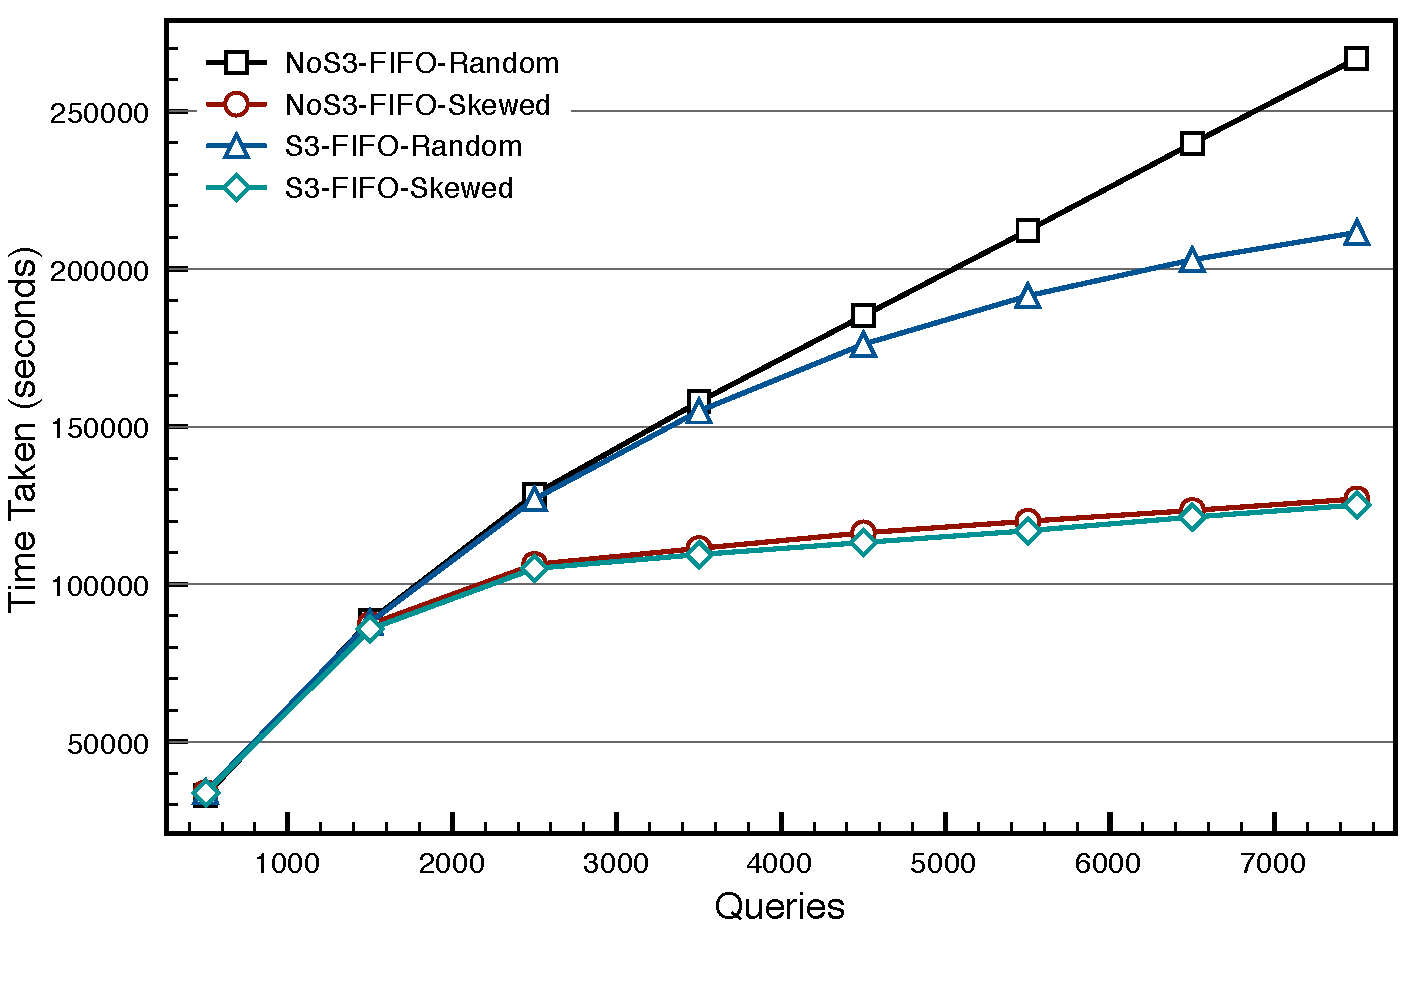
\includegraphics[width=3.2in, trim = 0mm 10mm 0mm 0mm, clip]{figures/time-cache-fifo-5mb.pdf}
  }
  \subfigure[25MB data files]{\
    \label{fig:time-cache-fifo-25mb}
    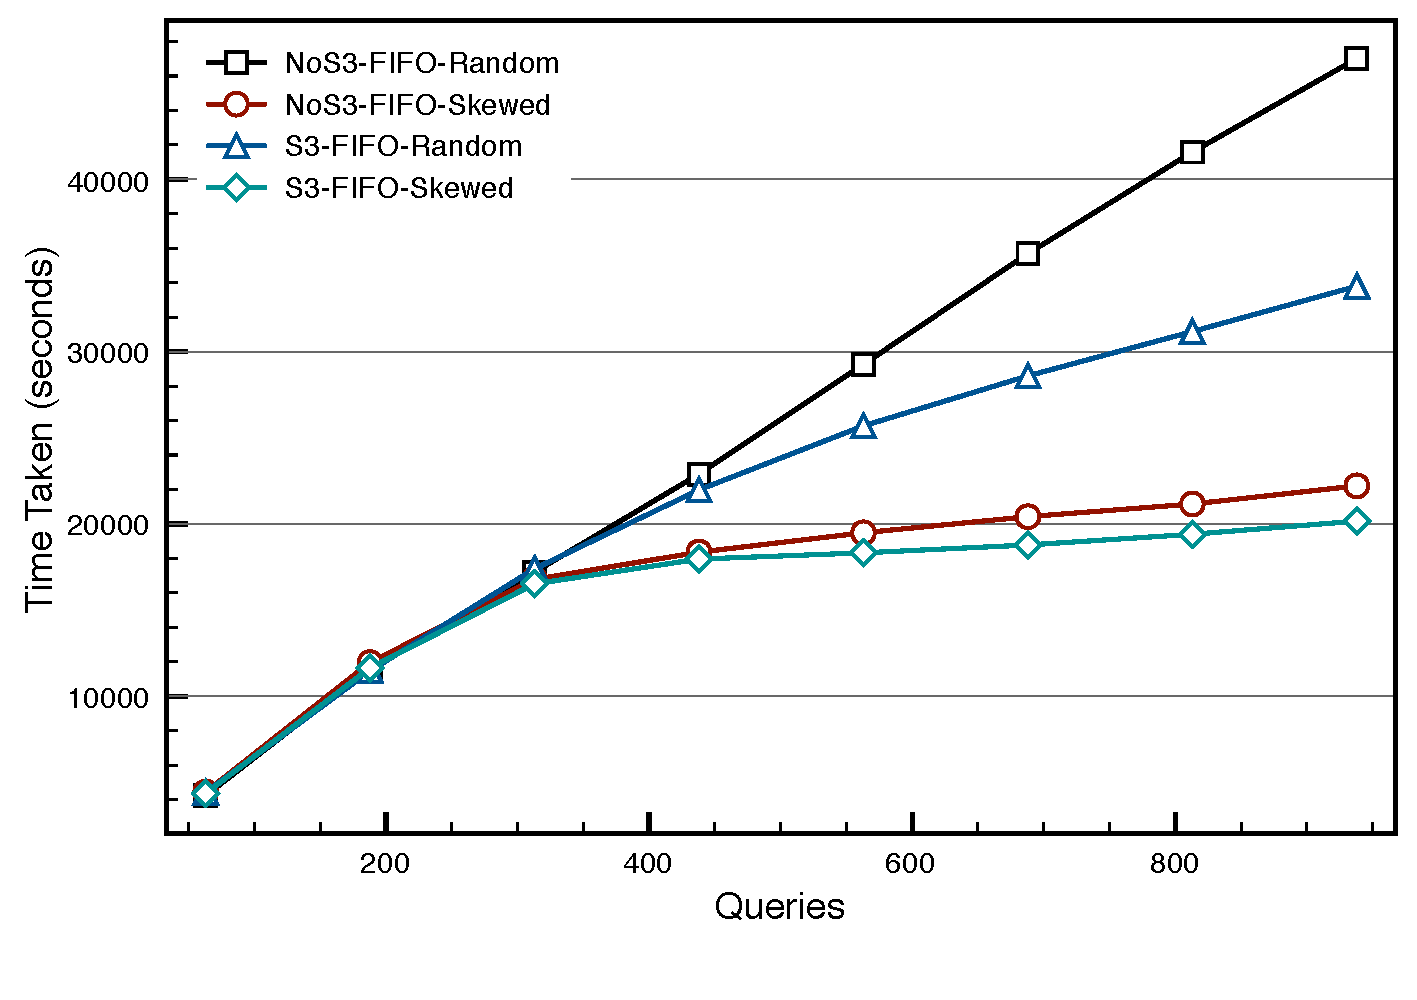
\includegraphics[width=3.2in, trim = 10mm 20mm 0mm 0mm, clip]{figures/time-cache-fifo-25mb.pdf}
  }
  \caption{Time taken using FIFO eviction strategy}
  \label{fig:time-cache-fifo}
\end{figure}

\begin{figure}
  \centering
  \subfigure[5MB data files]{\
    \label{fig:time-cache-lru-5mb}
    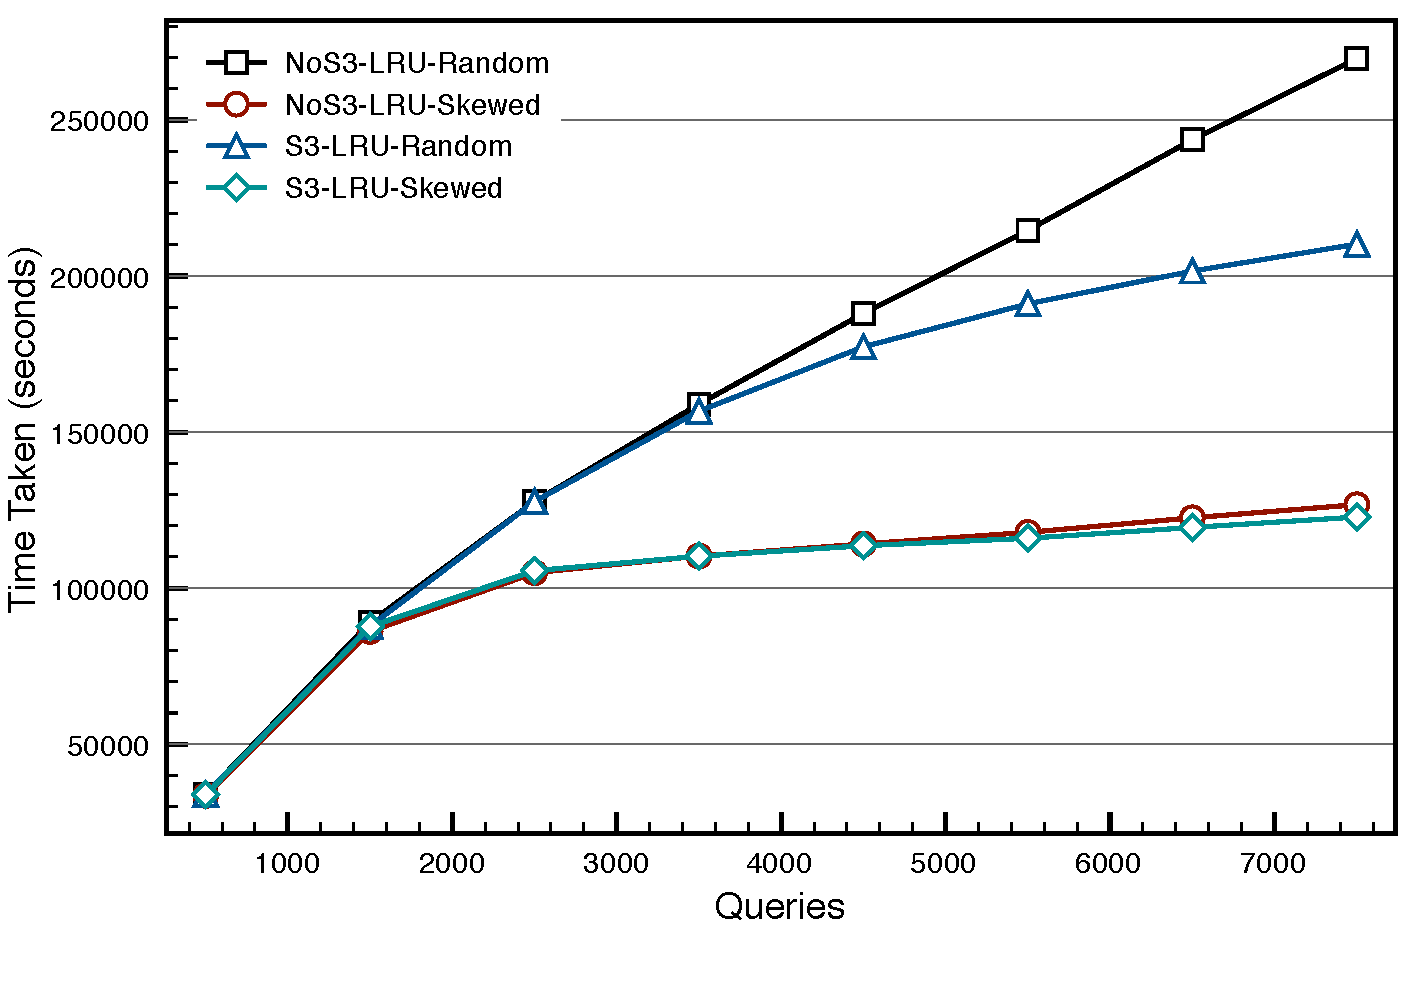
\includegraphics[width=3.2in, trim = 9mm 20mm 0mm 0mm, clip]{figures/time-cache-lru-5mb.pdf}
  }
  \subfigure[25MB data files]{\
    \label{fig:time-cache-lru-25mb}
    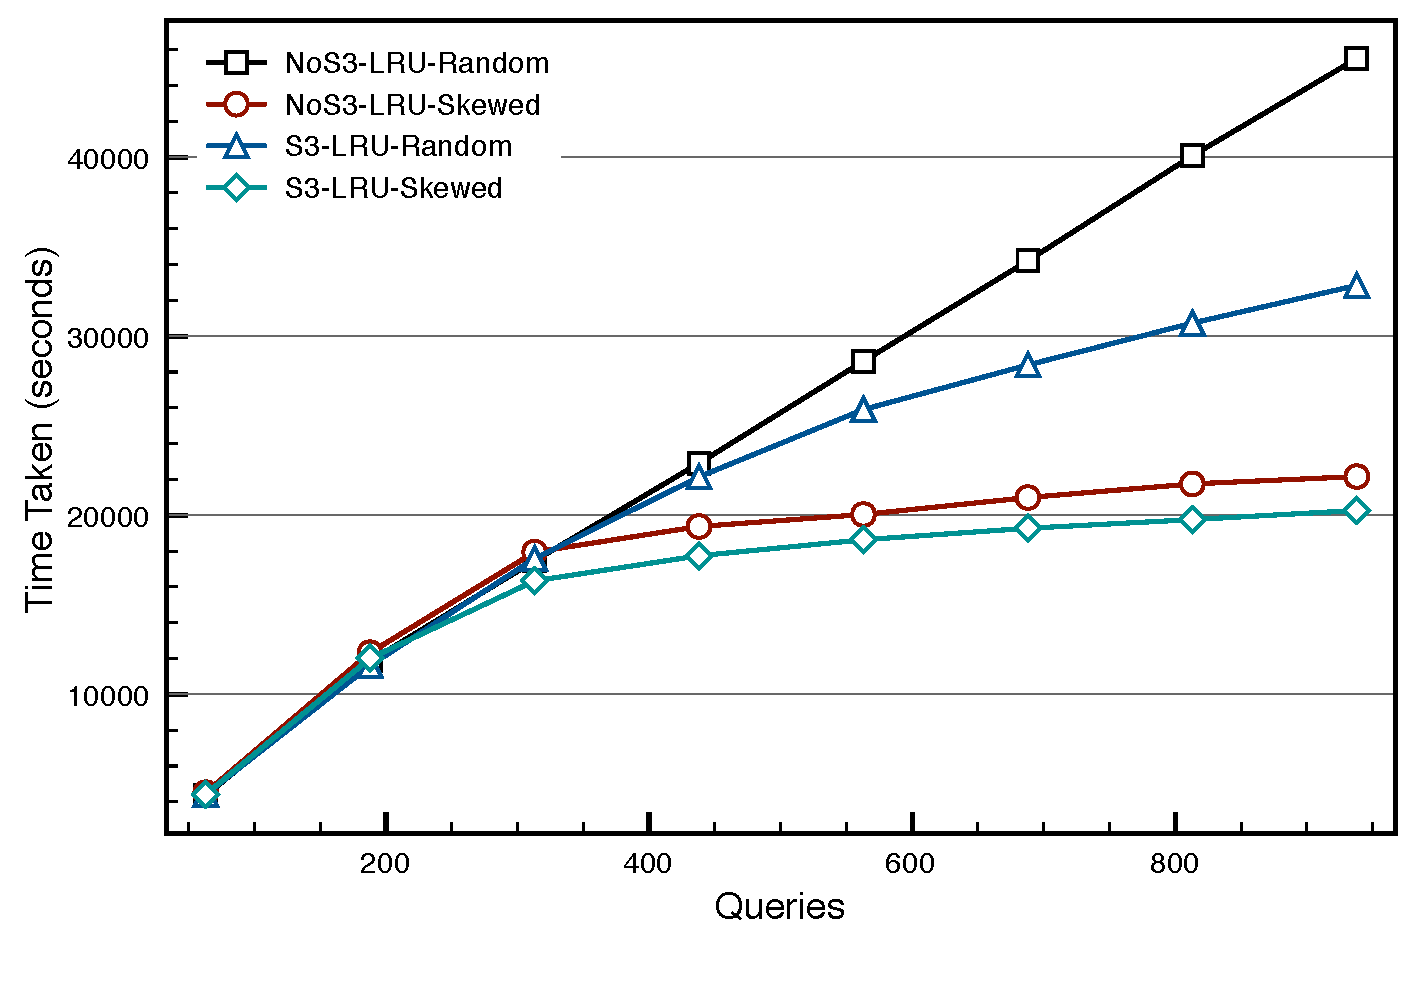
\includegraphics[width=3.2in, trim = 10mm 20mm 0mm 0mm, clip]{figures/time-cache-lru-25mb.pdf}
  }
  \caption{Time taken using LRU eviction strategy}
  \label{fig:time-cache-lru}
\end{figure}

\subsection{Execution Time}
To start, we compare the execution times of the various experimental
configurations outlined in Table~\ref{fig:experiment_configurations}. In
Figure~\ref{fig:time-cache-fifo}, we look at the eviction storage options: {\tt
S3} and {\tt None} for the distribution types using a simple {\tt FIFO}
eviction strategy. As expected, the skewed distributions execute in
significantly less time regardless of their storage options. This is due, in
both cases, to the fact that 10\% (the skewed portion upon which 90\% of
queries fall) of the key range is well within the bounds of the threshold (300
and 50 keys accordingly). As an additional result, we do not see {\tt S3}
providing quite so large a benefit as with the random distribution---with the
small set of keys retained in-memory for the last half of queries, its benefit
only plays out for the first half---shaving off approximately 2,000 seconds (33
minutes) in both the case of the {\tt 5MB} (1.5\%) and {\tt 25MB} (10\%).

That said, the benefit for randomly distributed queries \emph{is} quite large.
With {\tt 5MB} data files, we see a difference of 55,000 seconds (15.3 hours),
a 21\% decrease in time taken. For {\tt 25MB} data files, we peel off 13,200
seconds (3.7 hours), or approximately 28\%.

In Figure~\ref{fig:time-cache-lru}, we make notice of the same patterns using
the {\tt LRU} eviction strategy. With the {\tt 5MB} files, {\tt S3} shaves off
approximately 60,000 seconds (16.5 hours or 22\%) for the random distribution
and 4,000 seconds (1.1 hours or 3\%) for the skewed distribution. Finally, with
{\tt 25MB} files, we see a reduction of 12,600 seconds (3.5 hours or 28\%) and
1,900 seconds (32 minutes or 8\%) for random and skewed distributions
respectively.

\begin{figure}
  \centering
  \subfigure[5MB data files]{\
    \label{fig:missrates-cache-5mb}
    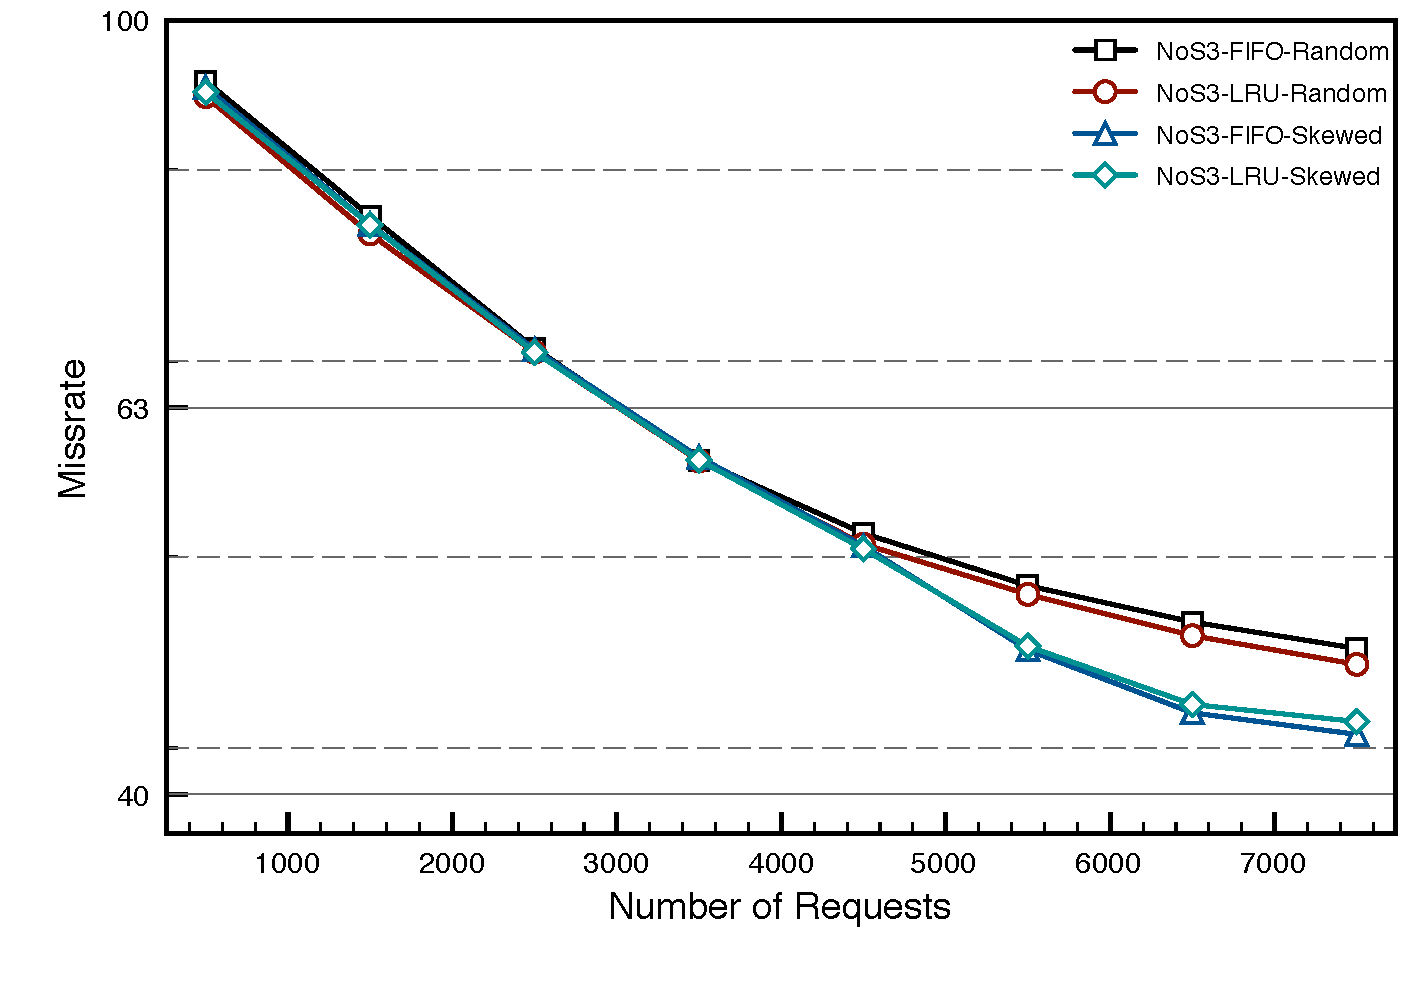
\includegraphics[width=3.2in, trim = 9mm 10mm 0mm 0mm, clip]{figures/missrates-cache-5mb.pdf}
  }
  \subfigure[25MB data files]{\
    \label{fig:missrates-cache-25mb}
    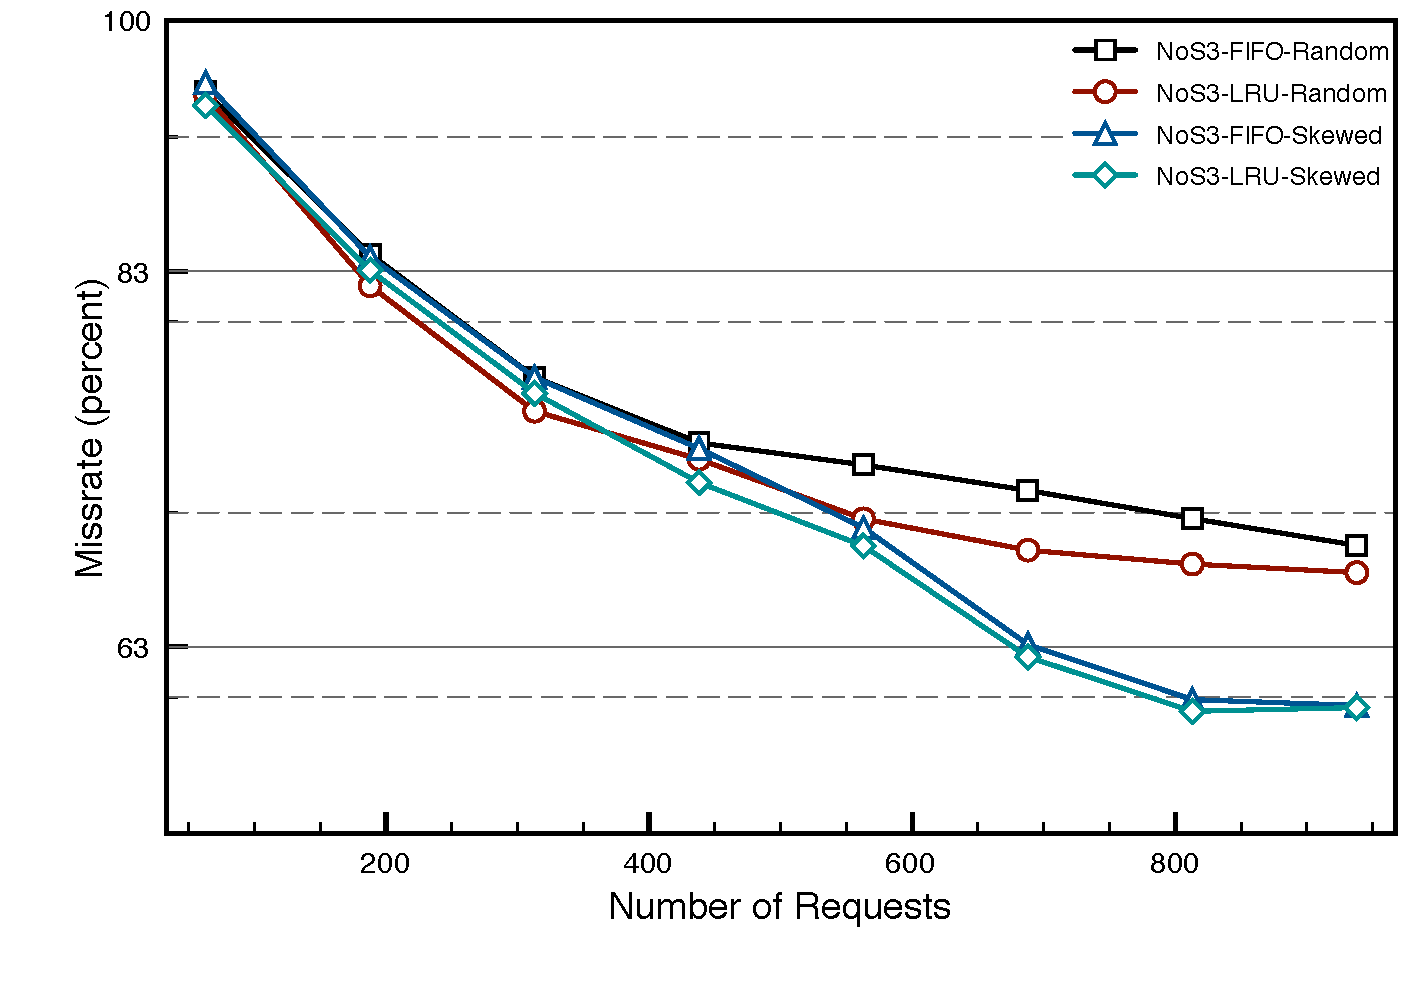
\includegraphics[width=3.2in, trim = 18.5mm 20mm 0mm 0mm, clip]{figures/missrates-cache-25mb.pdf}
  }
  \caption{Missrates by eviction strategy}
  \label{fig:missrate-cache}
\end{figure}

\begin{figure}
  \centering
  \subfigure[5MB data files]{\
    \label{fig:missrates-storage-5mb}
    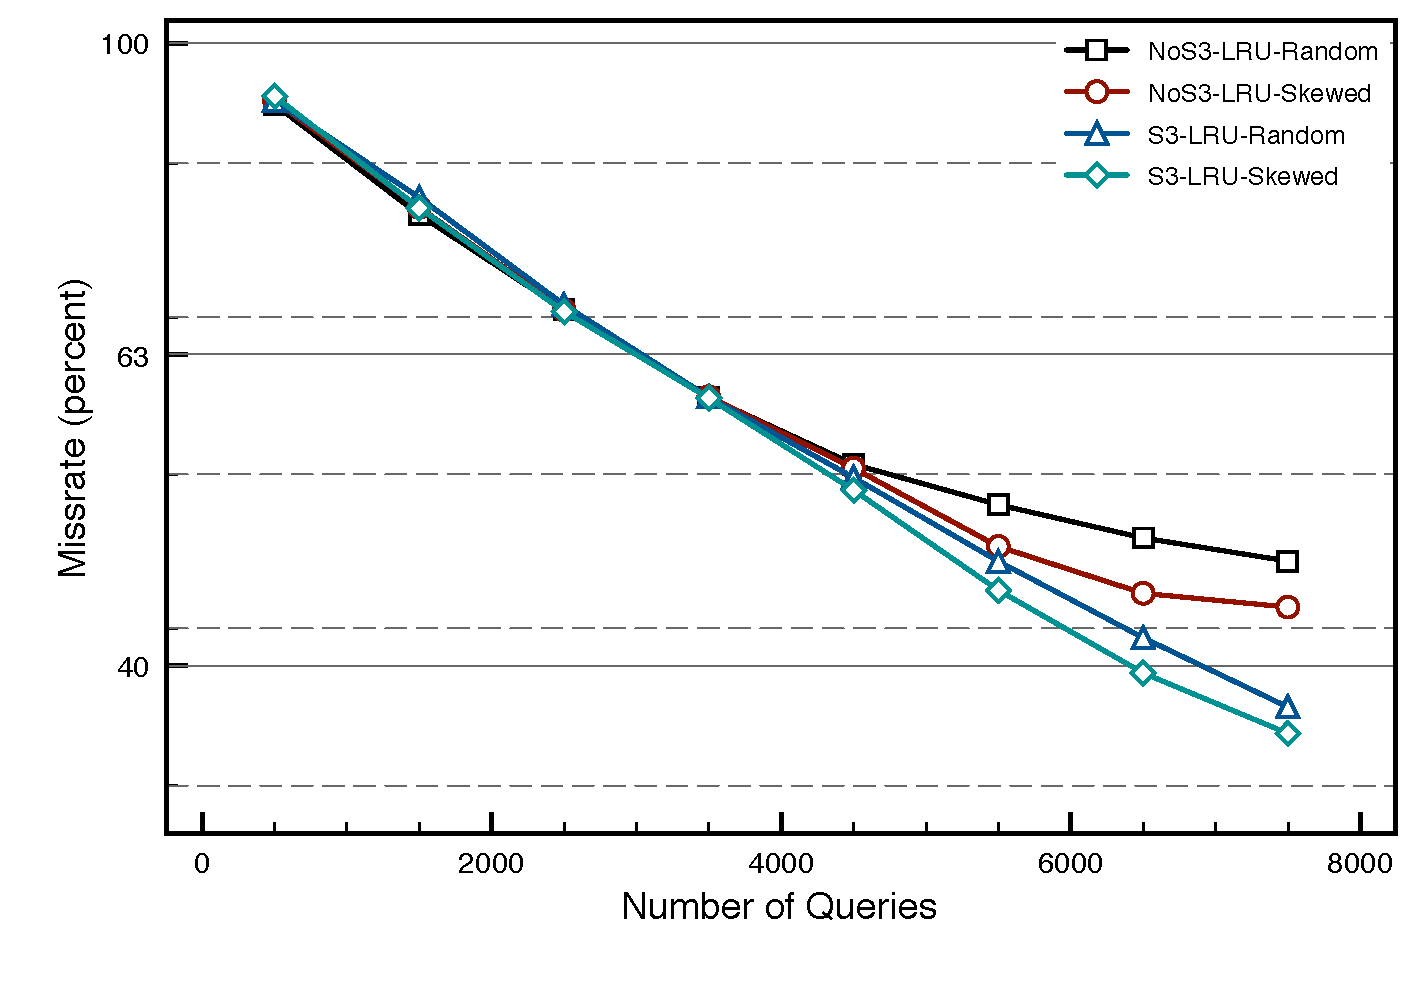
\includegraphics[width=3.2in, trim = 18mm 20mm 0mm 0mm, clip]{figures/missrates-storage-5mb.pdf}
  }
  \subfigure[25MB data files]{\
    \label{fig:missrates-storage-25mb}
    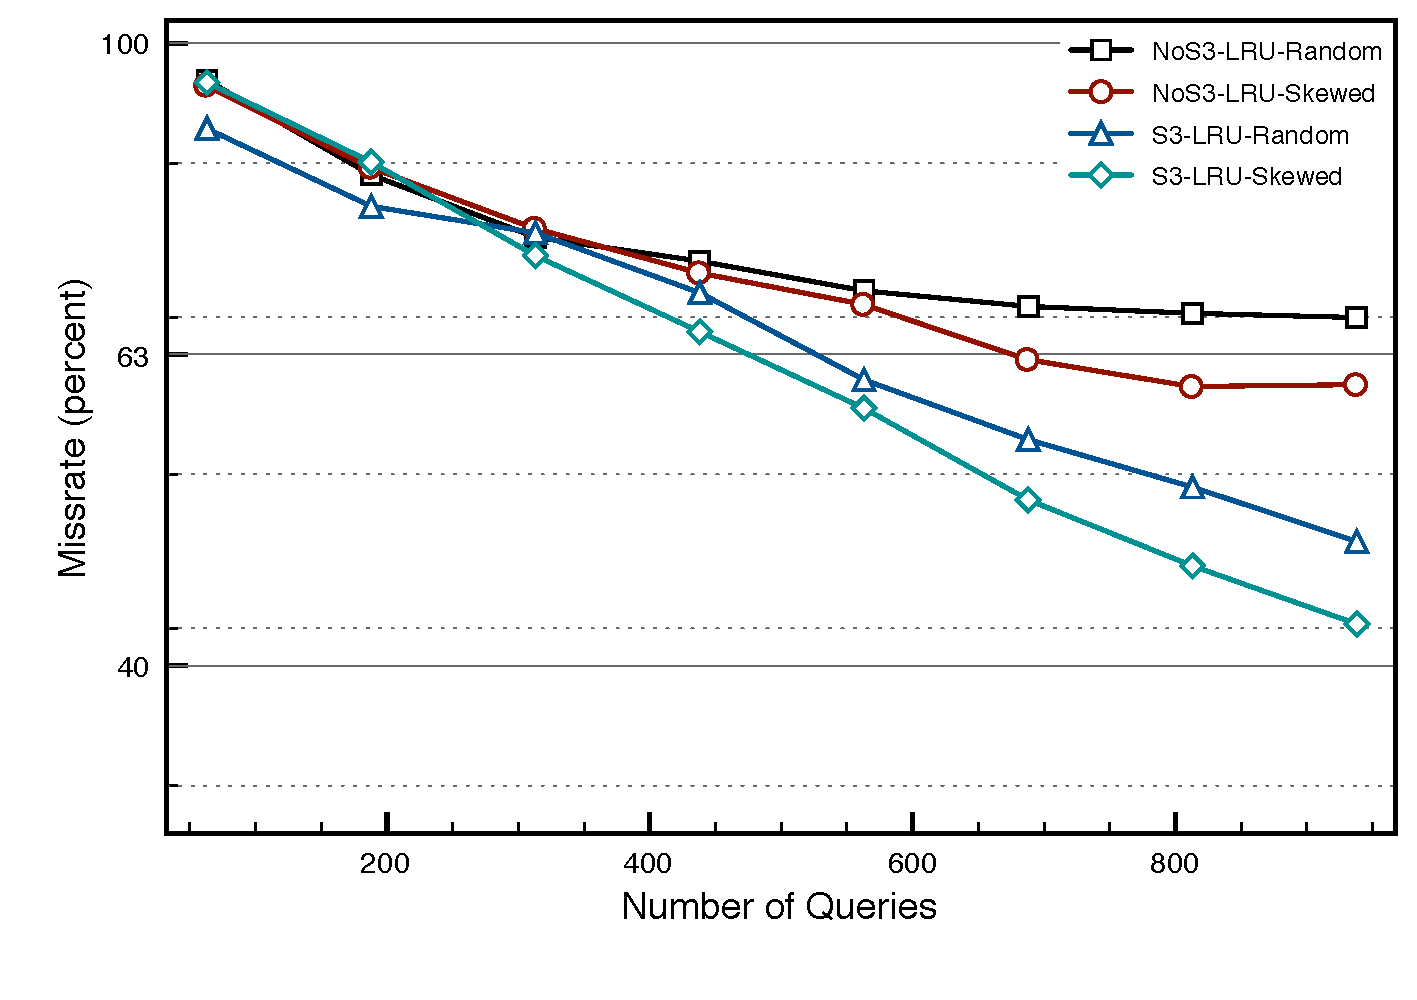
\includegraphics[width=3.2in, trim = 18mm 20mm 0mm 0mm, clip]{figures/missrates-storage-25mb.pdf}
  }
  \caption{Missrates by eviction storage}
  \label{fig:missrate-storage}
\end{figure}

\subsection{Missrate}
To give a broader sense of how these parameters affect the system we now
inspect the varying miss rates. As one would expect, lower miss rates
correspond to faster running times, and the greater storage capacity of the
{\tt S3}-backed configurations facilitate that. Similarly, skewed distributions
result in lower miss rates regardless of eviction strategy as the data set's
size is significantly reduced for the duration of the skewing period.

Figure~\ref{fig:missrate-cache} displays the miss rates across the different
eviction strategies. Though eviction strategy seems to have little-to-no effect
for the {\tt 5MB} files, we do see slightly more pronounced differences with the
{\tt 25MB}.

In contrast, Figure~\ref{fig:missrate-storage} displays significant gains in
performance between {\tt NoS3} and {\tt S3}-backed configurations.
Simultaneously, it demonstrates the efficacy of {\tt LRU} with random and
skewed distributions.

\subsection{Eviction Method} % (fold)
Finally, to get an overview of the performance differences between LRU and
FIFO, we present Figures~\ref{fig:perf-NoS3} and~\ref{fig:perf-S3}. To compute
these comparisons, we create a performance factor that is computed as
$\frac{t_{fifo}}{t_{lru}}$ where $t_{fifo}$ and $t_{lru}$ are the retrieval
times for FIFO and LRU respectively. With this metric, values greater than
$1.0$ indicate that FIFO performed \emph{worse} than LRU, while values less
than $1.0$ indicate that FIFO performed \emph{better}.

As we can see in many cases the difference in performance is inconclusive at
best. Occasionally we can see LRU consistently outperforming FIFO as in the
case of Figures~\ref{fig:perf-S3}. However, in the case of
Figure~\ref{fig:perf-NoS3-5mb} the FIFO implementation outperforms LRU\@. This
inconclusiveness is not totally unexpected however.
Figures~\ref{fig:missrate-cache} demonstrate that the performance difference
between the two implementations is very small. We do see that with larger files
the difference is more noticeable earlier on into the Random and Skewed
distributions. For this reason, we suggest that LRU is the better general-case
eviction method.

\begin{figure}
  \centering
  \subfigure[5MB data files]{\
    \label{fig:perf-NoS3-5mb}
    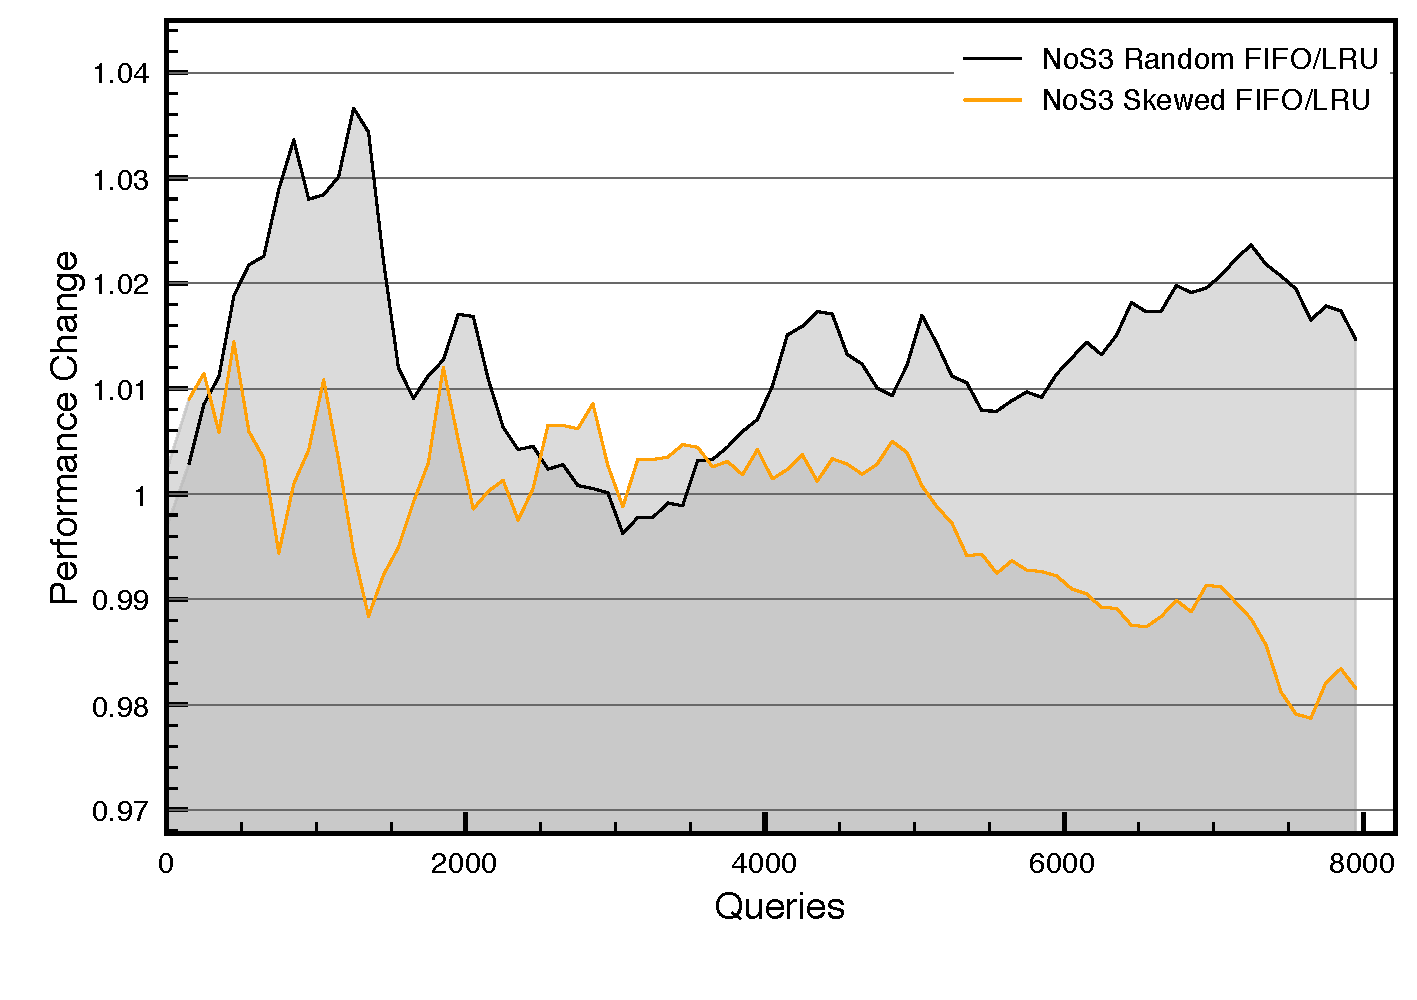
\includegraphics[width=3.2in, trim = 8mm 10mm 0mm 0mm,clip]{figures/FIFOvsLRU-NoS3-5mb.pdf}
  }
  \subfigure[25MB data files]{\
    \label{fig:perf-NoS3-25mb}
    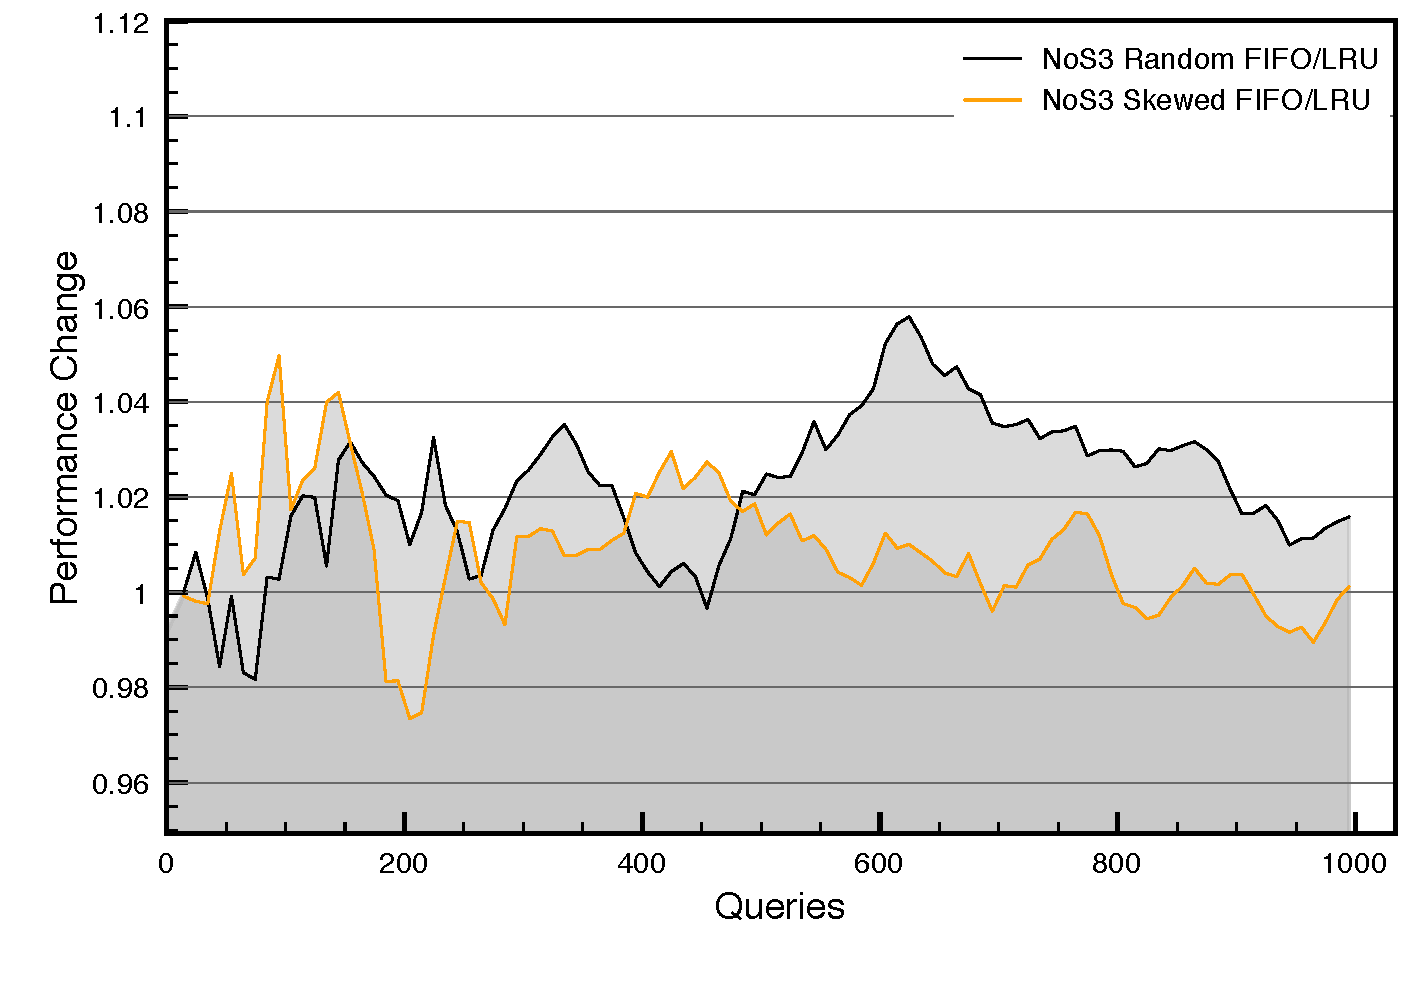
\includegraphics[width=3.2in, trim = 18.5mm 20mm 0mm 0mm,clip]{figures/FIFOvsLRU-NoS3-25mb.pdf}
  }
  \caption{Performance comparison without S3}
  \label{fig:perf-NoS3}
\end{figure}

\begin{figure}
  \centering
  \subfigure[5MB data files]{\
    \label{fig:perf-S3-5mb}
    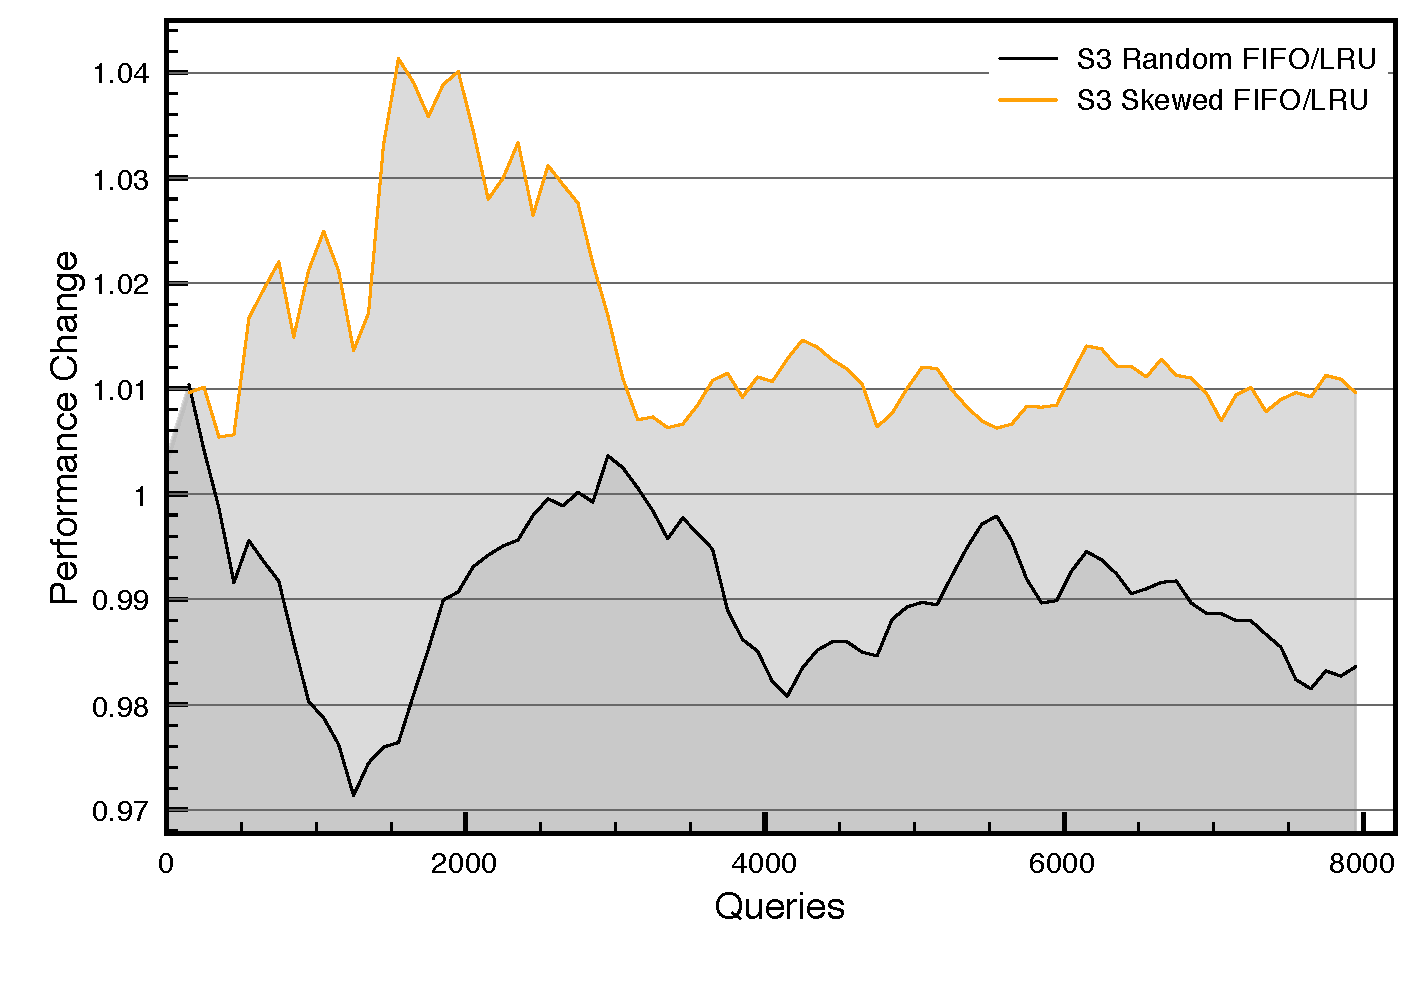
\includegraphics[width=3.2in, trim = 18.5mm 20mm 0mm 0mm,clip]{figures/FIFOvsLRU-S3-5mb.pdf}
  }
  \subfigure[25MB data files]{\
    \label{fig:perf-S3-25mb}
    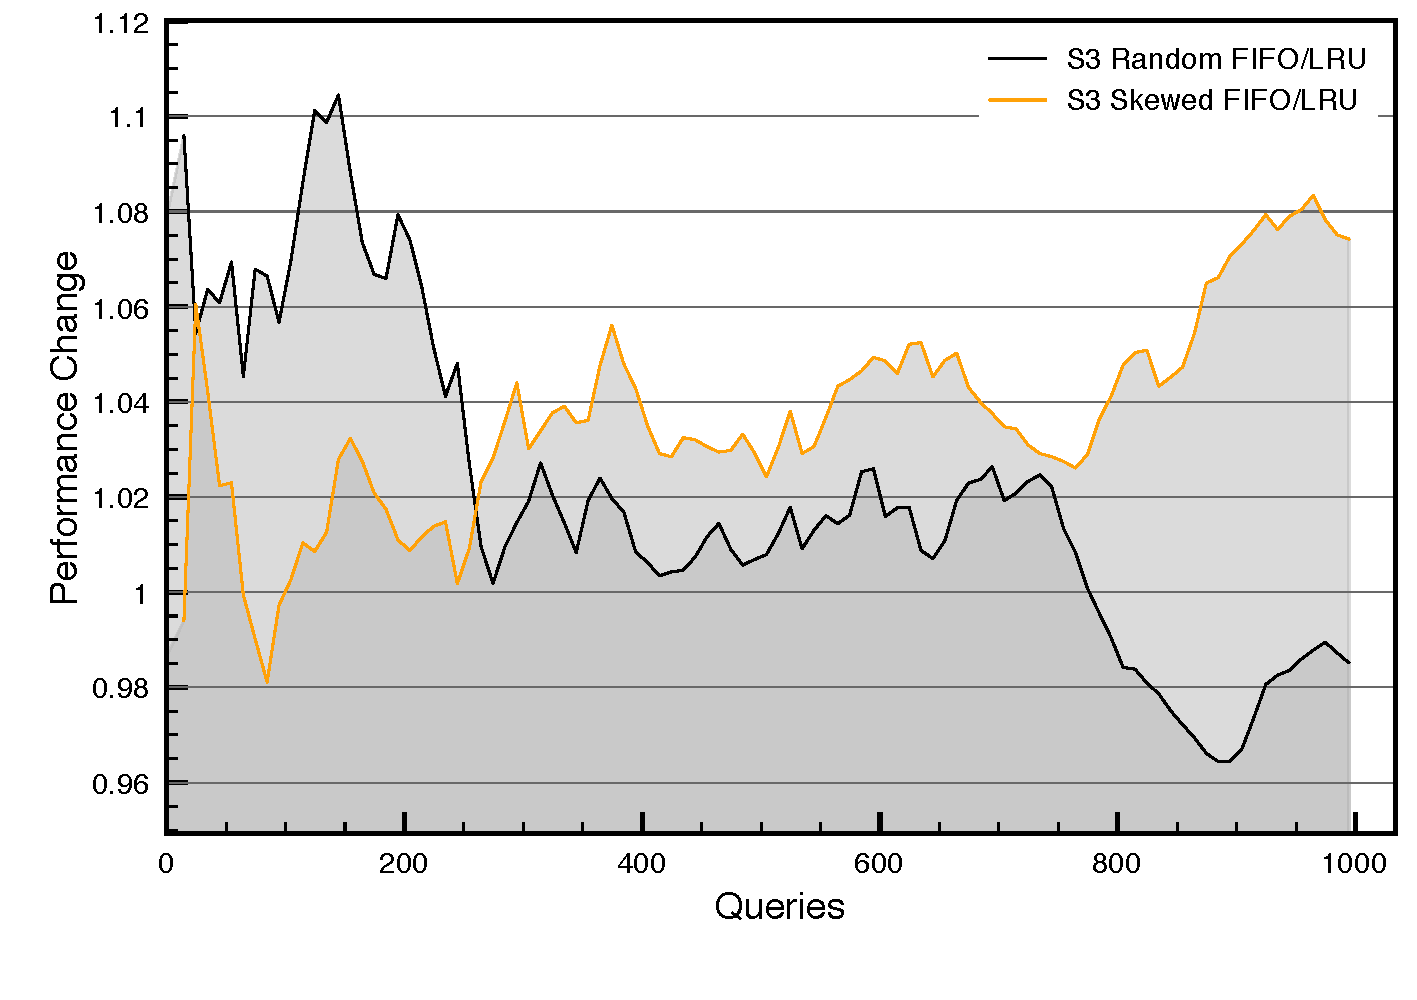
\includegraphics[width=3.2in, trim = 18.5mm 20mm 0mm 0mm,clip]{figures/FIFOvsLRU-S3-25mb.pdf}
  }
  \caption{Performance comparison with S3}
  \label{fig:perf-S3}
\end{figure}
% subsection Eviction Method (end)
% section results_eviction (end)
